\section{Beispiele}

In diesem Abschnitt werden verschiedene Berechnungsbeispiele aufgeführt.


\subsection{Berechnung der Entropie einer Quelle mit Gedächtnis}

Eine Quelle mit GEdächtnis kann mit einem Markoff-Diagramm dargestellt werden.
Diese Überlegungen und Berechnungen gelten auch für das Kanalmodell.

Bei Quellen mit Gedächtnis können wir ahnen, welches Zeichen als nächstes kommt,
daher sinkt der Informationsgehalt und die Redundanz nimmt zu.

\begin{tikzpicture}[->,>=stealth',shorten >=1pt,auto,node
                    distance=2.8cm,semithick]

	\node[state] (A)                    {$A$};
	\node[state] (B) [below left of=A]  {$B$};
	\node[state] (C) [below right of=A] {$C$};

	\path (A) edge [bend right] node [above left]  {$\sfrac{4}{5}$}  (B)
	          edge [bend left]  node               {$\sfrac{1}{5}$}  (C)
	      (B) edge [bend right] node [below right] {$\sfrac{1}{2}$}  (A)
	          edge [loop below] node               {$\sfrac{1}{2}$}  (B)
	      (C) edge [bend left]  node               {$\sfrac{1}{2}$}  (A)
	          edge [bend left]  node               {$\sfrac{2}{5}$}  (B)
	          edge [loop below] node               {$\sfrac{1}{10}$} (C)
	;

\end{tikzpicture}



\subsubsection*{1. Aufstellen der Matrix für die bedingte Wahrscheinlichkeit}

Die Werte können aus dem Diagramm ausgelesen werden.

\begin{tabular}[H]{|c|c|c|c|c|}
	\hline
	$p(y|x)$ & $Y=$ & $A$ & $B$ & $C$ \\
	\hline
	\multirow{3}{*}{$X=$} & $A$ geht über in & $0$ & $\frac{4}{5}$ & $\frac{1}{5}$ \\
	\cline{2-5}
	& $B$ geht über in & $\frac{1}{2}$ & $\frac{1}{2}$ & $0$ \\
	\cline{2-5}
	& $C$ geht über in & $\frac{1}{2}$ & $\frac{2}{5}$ & $\frac{1}{10}$ \\
	\hline
\end{tabular}


\subsubsection*{2. Berechnen der Wahrscheinlichkeit der einzelnen Zeichen}

Aufstellen der vier Gleichungen:

% TODO unterschied P vs p?
\begin{equation*}
	\begin{array}{rclclcl}
		1    &=& p(A)                   &+& p(B)                   &+& p(C) \\
		p(A) &=& p(A) \cdot 0           &+& p(B) \cdot \frac{1}{2} &+& p(C) \cdot \frac{1}{2} \\
		p(B) &=& p(A) \cdot \frac{4}{5} &+& p(B) \cdot \frac{1}{2} &+& p(C) \cdot \frac{2}{5} \\
		p(C) &=& p(A) \cdot \frac{1}{5} &+& p(B) \cdot 0           &+& p(C) \cdot \frac{1}{10}
	\end{array}
\end{equation*}

Daraus ergibt sich:
\begin{align*}
	p(A) &= \frac{1}{3} \\
	p(B) &= \frac{16}{27} \\
	p(C) &= \frac{2}{27}
\end{align*}


\subsubsection*{3. Zusammenfassen}

% TODO hä???
\begin{tabular}[H]{|c|c|c|c|c|}
	\hline
	$p(y|x)$ & $Y=$ & $A$ & $B$ & $C$ \\
	\hline
	\multirow{3}{*}{$X=$} & $A = \frac{1}{3}$ & $0 = 0$ & $\frac{4}{5} = \frac{4}{15}$ & $\frac{1}{5} = \frac{1}{15}$ \\
	\cline{2-5}
	& $B = \frac{16}{27}$ & $\frac{1}{2} = \frac{8}{27}$ & $\frac{1}{2} = \frac{8}{27}$ & $0 = 0$ \\
	\cline{2-5}
	& $C = \frac{2}{27}$ & $\frac{1}{2} = \frac{1}{27}$ & $\frac{2}{5} = \frac{4}{135}$ & $\frac{1}{10} = \frac{1}{135}$ \\
	\hline
\end{tabular}


\subsubsection*{4. Informationsgehalt der Zeichen}

Der Informationsgehalt berechnet sich wie folgt:
\[
	I(X_k) = \log_2\left(\frac{1}{p(x_k)}\right)
\]

Daraus ergibt sich:
{%
	\renewcommand{\arraystretch}{2}
	\begin{equation*}
		\begin{array}{rclcl}
			I(A) &=& \log_2\left(\frac{1}{\sfrac{1}{3}}\right) &=& 1.585 \, \textrm{Bit} \\
			I(B) &=& \log_2\left(\frac{1}{\sfrac{16}{27}}\right) &=& 0.755 \, \textrm{Bit} \\
			I(C) &=& \log_2\left(\frac{1}{\sfrac{2}{27}}\right) &=& 3.755 \, \textrm{Bit}
		\end{array}
	\end{equation*}
}%


\subsection{LZ78 Kompression}
\label{example:lz78}

Zu codierende Zeichenfolge: $00101110010110$

\subsubsection*{1. Aufteilen in eindeutige Zeichenfolgen}

\[
	0|01|011|1|00|10|11|0
\]

\subsubsection*{2. Übertragen}

\begin{minipage}{.4\linewidth}
	\begin{tabular}[H]{|l|l|}
		\hline
		0 & (0,0) \\
		\hline
		01 & (1,1) \\
		\hline
		011 & (2,1) \\
		\hline
		1 & (0,1) \\
		\hline
		00 & (1,0) \\
		\hline
		10 & (4,0) \\
		\hline
		11 & (4,1) \\
		\hline
		0 & (1) \\
		\hline
	\end{tabular}
\end{minipage}
\begin{minipage}{.6\linewidth}
	\tikzset{
	node/.style = {circle, draw=black, fill=white},
}

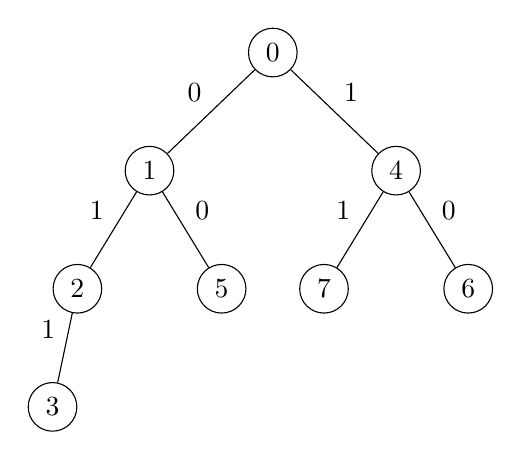
\begin{tikzpicture}
	\tikzstyle{level 1}=[sibling distance=25mm] 
	\tikzstyle{level 2}=[sibling distance=12mm] 
	\node[node]{0}
		child {
			node[node,left]{1}
			child {
				node[node,left]{2}
				child {
					node[node,left]{3}
					edge from parent node [above left] {1}
				}
				edge from parent node [above left] {1}
			}
			child {
				node[node,right]{5}
				edge from parent node [above right] {0}
			}
			edge from parent node [above left] {0}
		}
		child {
			node[node,right]{4}
			child {
				node[node,left]{7}
				edge from parent node [above left] {1}
			}
			child {
				node[node,right]{6}
				edge from parent node [above right] {0}
			}
			edge from parent node [above right] {1}
		}
	;
\end{tikzpicture}

\end{minipage}

\subsubsection*{3. Decodieren}

Bei jedem ankommenden Zeichenpaar wird der Baum bis zum entsprechenden Knoten
verfolgt und die Bits auf dem Weg ausgegeben. Danach wird bei Bedarf ein neuer
Knoten in den Baum eingefügt.

Beispiel (2,0):
\begin{itemize}
	\item Verfolgen des Baumes bis Knoten 2
	\item Ausgabe der Bits: $01$
	\item Anfügen eines neuen Knotens und Ausgabe des Weges dorthin: $0$
	\item Gesamte Bitfolge ist: $010$
\end{itemize}


\subsection{RSA}
\label{example:rsa}

\begin{description}
\item[Gegeben:] Primzahlen $p=11$ und $q=7$.
\item[Gesucht:] Schlüsselpaare $(e,N)$ und $(d,N)$.
\end{description}

Zuerst müssen $N$ und $\phi(N)$ berechnet werden:
\begin{align*}
	& N = p \cdot q \Rightarrow 11 \cdot 7 = 77 \\
	& \phi(N) = (p-1) \cdot (q-1) \Rightarrow 10 \cdot 6 = 60
\end{align*}
Nun wählt man ein $e$ kleiner als $N$ und teilerfremd zu $\phi(N)$.
\[
	e = 7
\]
Damit hat man schon den Public Key $(e,N)$. Jetzt muss man noch die Zahl $d$ für
den Private Key $(d,N)$ berechnen. Für $d$ muss gelten:
\[
	e \cdot d \bmod \phi(N) = 1
\]
Diese Gleichung löst man mit dem Erweiterten Euklidischen Algorithmus. Zuerst
multipliziert man $e$ so häufig dass das Produkt gerade noch $\leq \phi(N)$ ist
und addiert die Differenz $n$.
\[
\phi(N) = k \cdot e + n
\]
Bei der nächsten Gleichung setzt man jeweils für $\phi(N)$ $e$ ein und für $e$
$n$. Irgendwann wird $n=0$ und $e=1$. Mit Zahlen:
\begin{align}
	60 & = 8 \cdot 7 + 4 \label{eqn:rsa:ex1} \\
	7 & = 1 \cdot 4 + 3 \label{eqn:rsa:ex2} \\
	4 & = 1 \cdot 3 + 1 \label{eqn:rsa:ex3} \\
	3 & = 3 \cdot 1 + 0 \label{eqn:rsa:ex4}
\end{align}
Die letzte Gleichung benötigt man eigentlich nicht. Gleichung \ref{eqn:rsa:ex3}
kann man nun folgendermassen umschreiben:
\begin{equation}
\label{eqn:rsa:subs1}
	1 = 4 - 1 \cdot 3
\end{equation}
Gleichung \ref{eqn:rsa:ex2} kann als
\[
	3 = 7 - 1 \cdot 4
\]
geschrieben werden. Mit \eqref{eqn:rsa:ex2} kann die Zahl 3 in
\eqref{eqn:rsa:subs1} ersetzt werden.  
\begin{equation}
	1 = 4 - 1 \cdot (7 - 1 \cdot 4)
\end{equation}
Diese Gleichung muss man so umformen, dass die Zahl 4 ein Faktor des zweiten
Summanden ist, damit man sie danach wieder substituieren kann.
\begin{align}
	1 &= 4 - 7 + 4 \\
	1 &= \uminus 7 + 2 \cdot 4 \label{eqn:rsa:subs2}
\end{align}
Nun kann man \eqref{eqn:rsa:ex1} umformen und in \eqref{eqn:rsa:subs2}
einsetzen:
\begin{equation}
	1 = \uminus 7 + 2 \cdot (60 - 8 \cdot 7)
\end{equation}
Diese Gleichung muss jetzt so umgeformt werden, dass man etwas in der Form
\[
	1 = 60 \cdot k + 7 \cdot d
\]
bzw
\[
	1 = \phi \cdot k + e \cdot d
\]
erhält, weil damit die Bedingung $e \cdot d \bmod \phi(N) = 1$ erfüllt ist.
\begin{align}
1 & = \uminus 7 + 2 \cdot 60 - 16 \cdot 7 \\
1 & = 60 \cdot 2 - 16 \cdot 7 - 1 \cdot 7 \\
1 & = 60 \cdot 2 - 7 \cdot (16 + 1) \\
1 & = 60 \cdot 2 - 7 \cdot 17 \\
1 & = 60 \cdot 2 + 7 \cdot (\uminus 17)
\end{align}
Wenn $d$ negativ ist muss man noch $d \bmod N$ rechnen. Also $\uminus 17 \bmod
60 = 43$. Somit ist $d = 43$. Kontrolle:
\begin{alignat*}{3}
	e \cdot d & \bmod \phi(N) & \, = 1 \\
	7 \cdot 43 & \bmod \phi(60) & \, = 1
\end{alignat*}
